\section{The URDAD analysis and design process}

In this section we will introduce URDAD from the perspective of a quality driven process generating an analysis and design model which enforces certain model quality requirements.  URDAD\cite{solms_generating_2009} provides a service oriented analysis and design methodology, a metamodel introducing the semantics (modelling constructs) for an URDAD based domain specific language (the \emph{URDAD-DSL}), as well as a concrete text grammar which can be used to populate an URDAD model complying to the metamodel. A graphical grammar and diagram-based tooling around that grammar are under development. 

Services are recursively assembled from lower level services with leaf services representing services which are sourced from the environment. These may include persistence services, services sourced from the execution frameworks or implmentation languages, services sourced from off the external systems as well as manually executed services provided by business partners, business units, and so on.

The resultant URDAD model represents a \emph{Computation Independent Model} (CIM) as the services contracts and processes can be realized as system  or business contracts (SLAs) and system or manual processes respectively. Nevertheless, the model has a level of detail and preciseness which is generally associated with \emph{Platform Independent Models} (PIMs) and not commonly with CIMs as it contains testable service contracts and and implementable process specifications for services across levels of granularity.

%-----------------------------------------------------------

\subsection{Quality drivers employed by URDAD}

Most of the quality drivers discussed in \ref{sec:modelQualityDriversAndMetrics} are builts into the URDAD process. Table \ref{tab:qualityDrivers} lists the employed quality drivers and the model qualities they are meant to support.

\begin{table}[h]
 \caption{URDAD model quality drivers for quality requirements}
 \label{tab:qualityDrivers}
\begin{tabular}{|l|cc|cccccccc|} \hline
\multirow{4}{*}{\bf Quality driver} & \multicolumn{10}{c|}{\bf Model qualities} \\ \cline{2-11}
& & & \multicolumn{8}{c|}{Pragmatic model qualities}\\ \cline{4-11}
    & \begin{sideways}Semantic\end{sideways} & \begin{sideways}Syntactic\end{sideways}  & \begin{sideways}Simplicity\end{sideways}
    & \begin{sideways}Completeness\end{sideways} & \begin{sideways}Modifiability\end{sideways} & \begin{sideways}Consistency\end{sideways}
    & \begin{sideways}Decoupling\end{sideways} & \begin{sideways}Cohesion\end{sideways} & \begin{sideways}Reusability\end{sideways}
    & \begin{sideways}Traceability\end{sideways} \\ \hline
%                                       Semantic     Syntax        Simplicity  Completeness   Modifiable  Consistent  Decoupled    Cohesion     Reuse        Traceable
Metamodel and/or ontology              & \checkmark & \checkmark & \checkmark & \checkmark & \checkmark & \checkmark & \checkmark &            &            & \checkmark \\
Graphical and/or text grammar          &            & \checkmark & \checkmark &            & \checkmark &            &            &            &            
& \\
Fix levels of granularity              &            &            & \checkmark &            & \checkmark &            &            &            &
\checkmark & \checkmark \\ 
Enforce single reponsibility principle &            &            & \checkmark &            & \checkmark &            &            & \checkmark & \checkmark & \checkmark \\ 
Service dependency via contracts       &            &            & \checkmark &            & \checkmark &            & \checkmark &            & \checkmark & \checkmark \\ 
Testable pre- \& post-conditions       &            &            &            & \checkmark & \checkmark & \checkmark &            &            &            &  \\ 
Process localization in controller     &            &            & \checkmark &            & \checkmark &            & \checkmark & \checkmark & \checkmark & \checkmark \\ 
Traceability Links                     &            &            & \checkmark & \checkmark & \checkmark & \checkmark &            &            &            & \checkmark \\ \hline 
\end{tabular}
  
\end{table}

%------------------------------------------------------------------------

\subsection{The URDAD process}
\label{sec:urdadProcess}

\begin{enumerate}
 \item {\bf Requirements analysis} for level of granularity yielding service contract
  \begin{enumerate}
    \item Identify stakeholders for the services.
    \item For each stakeholder, identify functional requirements (pre- and post-conditions) and quality requirements for the service.
    \item Assess consistency of stakeholder requirements.
    \item Fix level of granularity by consolidating lower level pre- and post-conditions into higher level pre- and post-conditions. 
	  \emph{\textbf{\textit{Note:}} This includes the absorption of certain pre and/or post-conditions into encompassing pre- or post-conditions and the identification of a higher level pre- or post-condition which groups the some of the specified pre- and/or post-conditions into a higher level functional requirement addressing a at some level of granularity a single responsibility (enforcing the single responsibility principle). The purpose of this process is to project out levels of granularity in a repeatable way, simplifying the process at a particular level of granularity and improving reuse and cohesion.}
    \item Specify data structure for request and result classes.
    \item Formalize the pre and post-conditions by specifying the user test process for each and for each pre-condition the exception which will be raised if the pre-condition is not met.
    \item Identify the responsibility domain for the service and assign the services contract to that responsibility domain making sure that an appropriate service contract has not already been assigned to that responsibility domain. 
  \end{enumerate}

 \item {\bf Process design} for level of granularity defining a service implementation.
      \begin{enumerate}
	\item Assess whether the requested service falls within scope for the context (e.g.\ system, system component, organization, business unit, \dots).
	\item Check within the responsibility domain of the service whether realizing the services contract. If so return that service.
        \item Identify for each functional requirement an abstract service (in the form of a service contract) to be used to address that functional requirement.
	\item If a new service is defined, assign it to the appropriate responsibility domain, ensuring cohesion of the responsibility domain. \emph{\textbf{\textit{Note:}} Responsibility domains contain lower level responsibility domains and the service needs to be assigned to a responsibility domain at the appropriate level of granularity.}
	\item Choreograph the process across the abstract services used to address the functional requirements with each pre-condition assessment leading potentially leading to a terminal activity of raising an exception and all other paths leading to the terminal activity of returning the result object. \emph{\textbf{\textit{Note:}} The services across levels of granularity are decoupled through services contracts.}
      \end{enumerate}

  \item Recursively repeat the process for each lower level service which is not available.
\end{enumerate}

%\missingfigure{URDAD process}

The methodology does not envisage that a single requirements engineer does the requirements and process design across levels of granularity. Instead requirements engineers specializing in different responsibility domains (e.g.\ business analysts across business units of the organization) collaborate to define the complete requirements model.

%------------------------------------------------------------------------

\subsection{The URDAD metamodel and text grammar}
\label{sec:urdadDsl}

URDAD does not prescribe the language which should be used to encode the requirements and process model representing OMG's CIM, but it provides the option of using a domain specific language for URDAD, the \emph{URDDAD-DSL}. URDAD require, however, that the modelling language used supports the semantics for specifying 1) \emph{services contracts} with pre- and post-conditions, quality requirements and data structure specification for the inputs and outputs, 2) parametrized state constraints applying to service environment, 3) object-oriented data structure specification, 4) service specification including 5a) the specification of which service is used to address which functional requirement and 5b) the process specification in the form of a choreography across lower level services and 6) the assigning of model artifacts including services contract and service specifications to responsibility domains. URDAD also requires the linkage between a requirement and the stakeholder who requires it. The stakeholder can be a responsibility domain or a service.

Historically UML together with OCL and an URDAD profile were used with services contracts represented by interfaces, pre- and post-conditions and quality requirements by constraints, data structure specifications by class diagrams and process choreography specified in activity diagrams assigned to service implementation within classes. The activity diagrams were allowed to only use call operations and control logic. The approach was, however, tedious and error prone and the resultant models were seldom in a state which allowed for model transformation, code and test generation and solid documentation generation. Furthermore, additional semantic relationships, not all of which could be represented in diagrams, needed to be added. Full testable service contract specification and complete process specification facilitating full test and code generation proved particularly challenging.

Another modeling language commonly used, particularly in the context of service oriented process specification, is the \emph{Business Process Modeling Notation}. However, it suffers from being too technical\cite{fouad_embedding_2010} and needs to be supplemented by UML or other languages to allow for full data structure and service contract specification. Many UML tool vendors make BPMN available as a UML profile, enabling the integration of BPMN process specification with other UML modeling elements and diagrams. This approach, however, effectively increases the already substantial size of the UML even further, resulting in further learning costs and inconsistency risks.

In order to simplify the URDAD model encoding and to improve the quality of URDAD models an URDAD metamodel and text grammar have been sepcified (a separate paper entitles \emph{`A Domain-Specific Language for URDAD Based Requirements Elicitation'} is currently being reviewed. Here we discuss aspects of the metamodel and text grammar from a quality perspective. In particular, many of the model qualities are either enforced or supported through the metamodel including
\begin{itemize}
 \item decoupling of services across levels of granularity through services contracts,
 \item a range of traceability links including enforced usage of both satisfiability links and \emph{`requiredBy'} links between requirements and stakeholders,
 \item the assignment of services into responsibility domains, and 
 \item the support of parametrized, reusable constraints for the specification of pre- and post-conditions as well as guard conditions for conditional functional requirements and alternative flows within processes.
\end{itemize}

The URDAD metamodel is modularized with a \emph{core module} introducing base concepts like that of a model, an element, a responsibility domain and an expression. A {\emph data module} introduces standard modeling constructs for object-oriented data specification. More interesting is the constraints module which introduces modelling constructs through which one can specify reusable parametrized constraints which are applicable to a services oriented approach.

Constraints are required for the specification of functional requirements (pre- and post-conditions), data structure constraints and decision points in processes. Note that the same constraint can be a pre-condition for some services, a post-condition for other services and a guard condition within a conditional flow of a process. The Object-Constraint Language (OCL)\cite{_object_2010}  has become the de-facto standard for specifying constraints across object graphs. However, in a services-oriented approach and in the context of reusable, parametrised constraints the OCL alone is not expressive enough. This is due to two reasons.

Firstly, in a service-oriented context the actual environmental state is only accessible through services which report on the environment and not by traversing an object graph. The specification of constraints must thus relate to the specification of services through which information is sourced from the environment together with a set of data structure constraints on the obtained information. OCL can be used for the latter, but is insufficient for the complete specification of a constraint.

Secondly, the definition of reusable constraints requires support for binding parameters. \emph{For example}, assume a constraint that some `Person' must be `registered'. Such a constraint can contribute to pre- or post-conditions of services. Hence, to be able to do so, the person identifier would have to be passed as a parameter to the constraint entity. 

The following listing shows an simple example of a parametrized constraint, \emph{studentEnrolledForPresentation}, which demonstrated that a state constraint is assembled from a process that extracts information from the environment and a set of data constraints applied to the obtained information.
\lstset{language=urdad,caption=Specifying a state constraint in the URDAD text grammar.,label=constraintTextSyntax}
\begin{lstlisting}[numbers=left,escapechar=|]
StateConstraint studentEnrolledForPresentation receiving Variable enrollForPresentationRequest ofType EnrollForPresentationRequest
{
  stateAssessmentProcess doSequential
  {
    create Variable getEnrollmentsRequest ofType GetEnrollmentsRequest
    set Query OCL:"getEnrollmentsRequest.presentationIdentifier" equalTo Query OCL:"enrollForPresentationRequest.presentationIdentifier"
    requestService getEnrollments with getEnrollmentsRequest yielding Variable getEnrollmentsResult ofType GetEnrollmentsResult
  }
  Constraint OCL:"getEnrollmentsResult.enrollments.includes (enrollForPresentationRequest.personIdentifier)"
}
\end{lstlisting}

Figure \ref{fig:constraintModule}, shows the elements provided with the constraints module of the URDAD metamodel as well as their relationship with other modeling constructs.
\begin{figure}[Htbp]
  \centering
  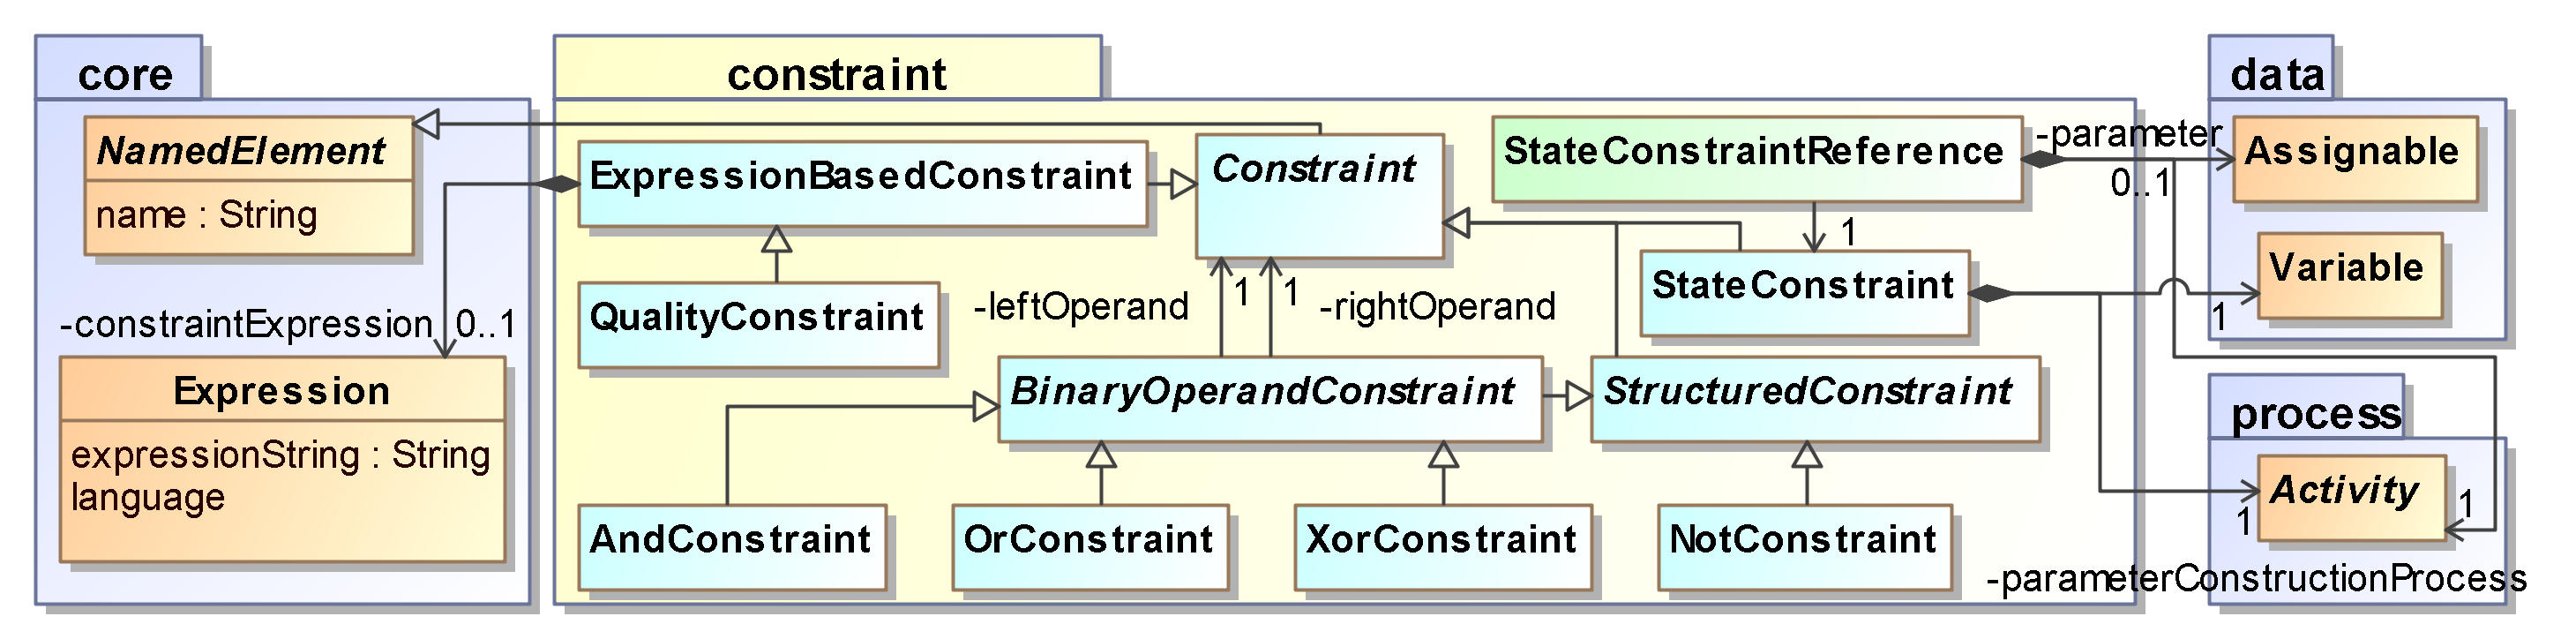
\includegraphics{constraint}
  \caption{The modeling constructs available in URDAD facilitating the specification of constraints}
  \label{fig:constraintModule}
\end{figure}

The \emph{contract module} of the URDAD metamodel has the modeling constructs used to specify services contracts including \emph{requiredBy} links between requirements and stakeholders. The specification of a services contract within the URDAD DSL text grammar is illustrated with the following listing.
\lstset{language=urdad,caption=Specifying a service contract in the textual URDAD DSL syntax.,label=contractTextSyntax}
\begin{lstlisting}[numbers=left,escapechar=|]
ServiceContract enrollForPresentation
{
   FunctionalRequirements receiving Variable enrollForPresentationRequest ofType EnrollForPresentationRequest
   {
      PreCondition enrollmentPrerequisitesMet requiredBy (TrainingRegulator Student) raises EnrollmentPrerequisitesNotSatisfiedException checks constraint enrollmentPrerequisitesForPresentationMet with ValueOf enrollForPresentationRequest
      PostCondition enrollmentProcessPerformed requiredBy (Student Client TrainingRegulator) ensures constraint studentEnrolledForPresentation          with ValueOf studentEnrolledRequest constructedUsing doSequential
         {
            create Variable studentEnrolledRequest ofType StudentEnrolledRequest
            set Query OCL:"studentEnrolledRequest.personIdentifier" equalTo Query OCL:"enrollForPresentationRequest.personIdentifier"                            
            set Query OCL:"studentEnrolledRequest.presentationIdentifier" equalTo Query OCL:"enrollForPresentationRequest.presentationIdentifier"                            
         }  
      PostCondition invoiceIssued ...
    }            
    Request DataStructure EnrollForPresentationRequest 
    {
       has identification presentationIdentifier identifying Presentation
       has identification studentIdentifier identifying Person
       has identification clientIdentifier identifying LegalEntity         
    }
    Result DataStructure EnrollForPresentationResult 
    {
       has component proofOfEnrollment ofType ProofOfEnrollment
       has component invoice ofType Invoice
       has component studyGuide ofType StudyGuide
    }
}
\end{lstlisting}

The contract specification includes pre- and post-conditions, quality requirements and the data structure specifications for the request and result objects of the service. Figure \ref{fig:contractModule} shows the elements of the contract modules of the URDAD metamodel.

\begin{figure}[Htbp]
  \centering
  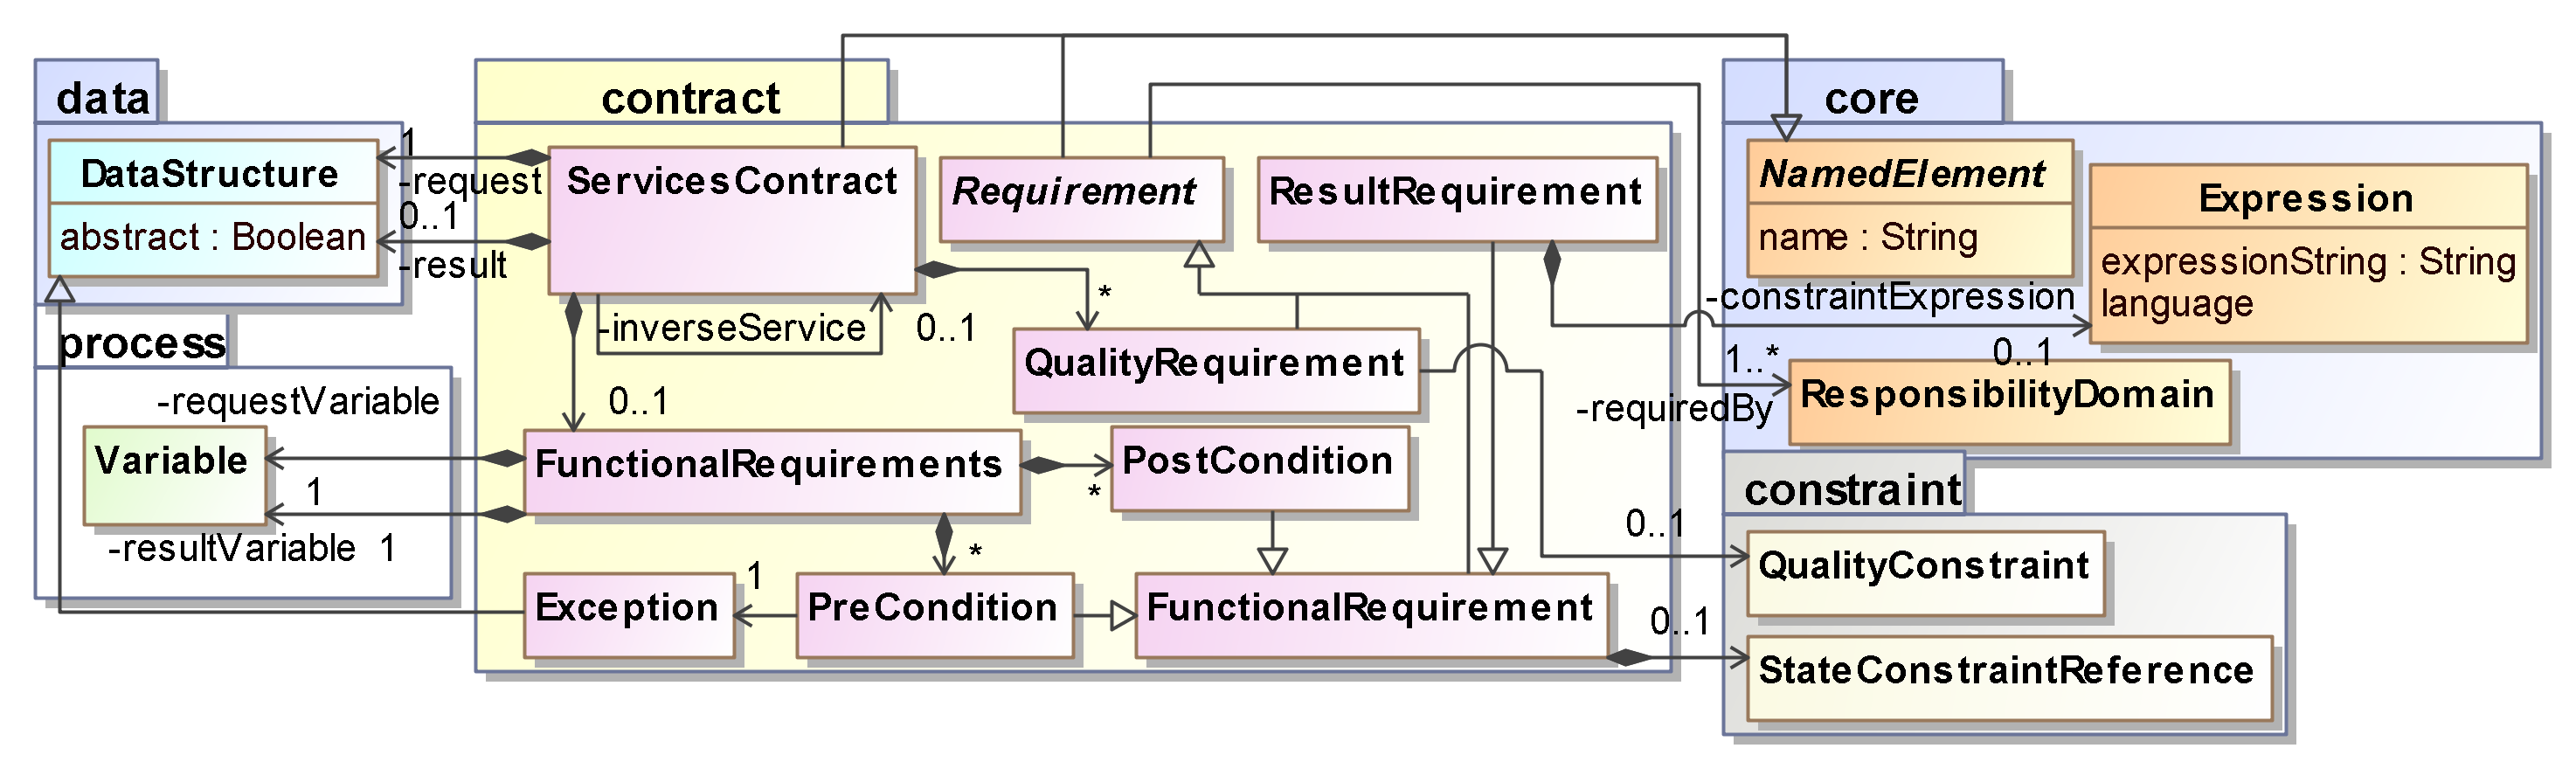
\includegraphics{contract}
  \caption{The modeling constructs available within URDAD to specify services contracts.}
  \label{fig:contractModule}
\end{figure}

The \emph{process module} depicted \ref{fig:processModule} in figure contains the specification of the services used to address the functional requirements and the process specification for the service. The metamodel enforces realization links between a lower level abstract service (service contract) which is used in a process and the functional requirement for which the lower level service is used. These links are manifested as \verb+usedToAddress+ links representing satsifaction links of \cite{ramesh_toward_2001}). 

The service process is specified as a choreography across the lower level services used to address the functional requirements and supports control constructs, process state management, the handling exceptions raised by lower level services, activities for raising an exception associated with a pre-condition of the service, and the return of a result object for the service. 

\begin{figure}[Htbp]
  \centering
  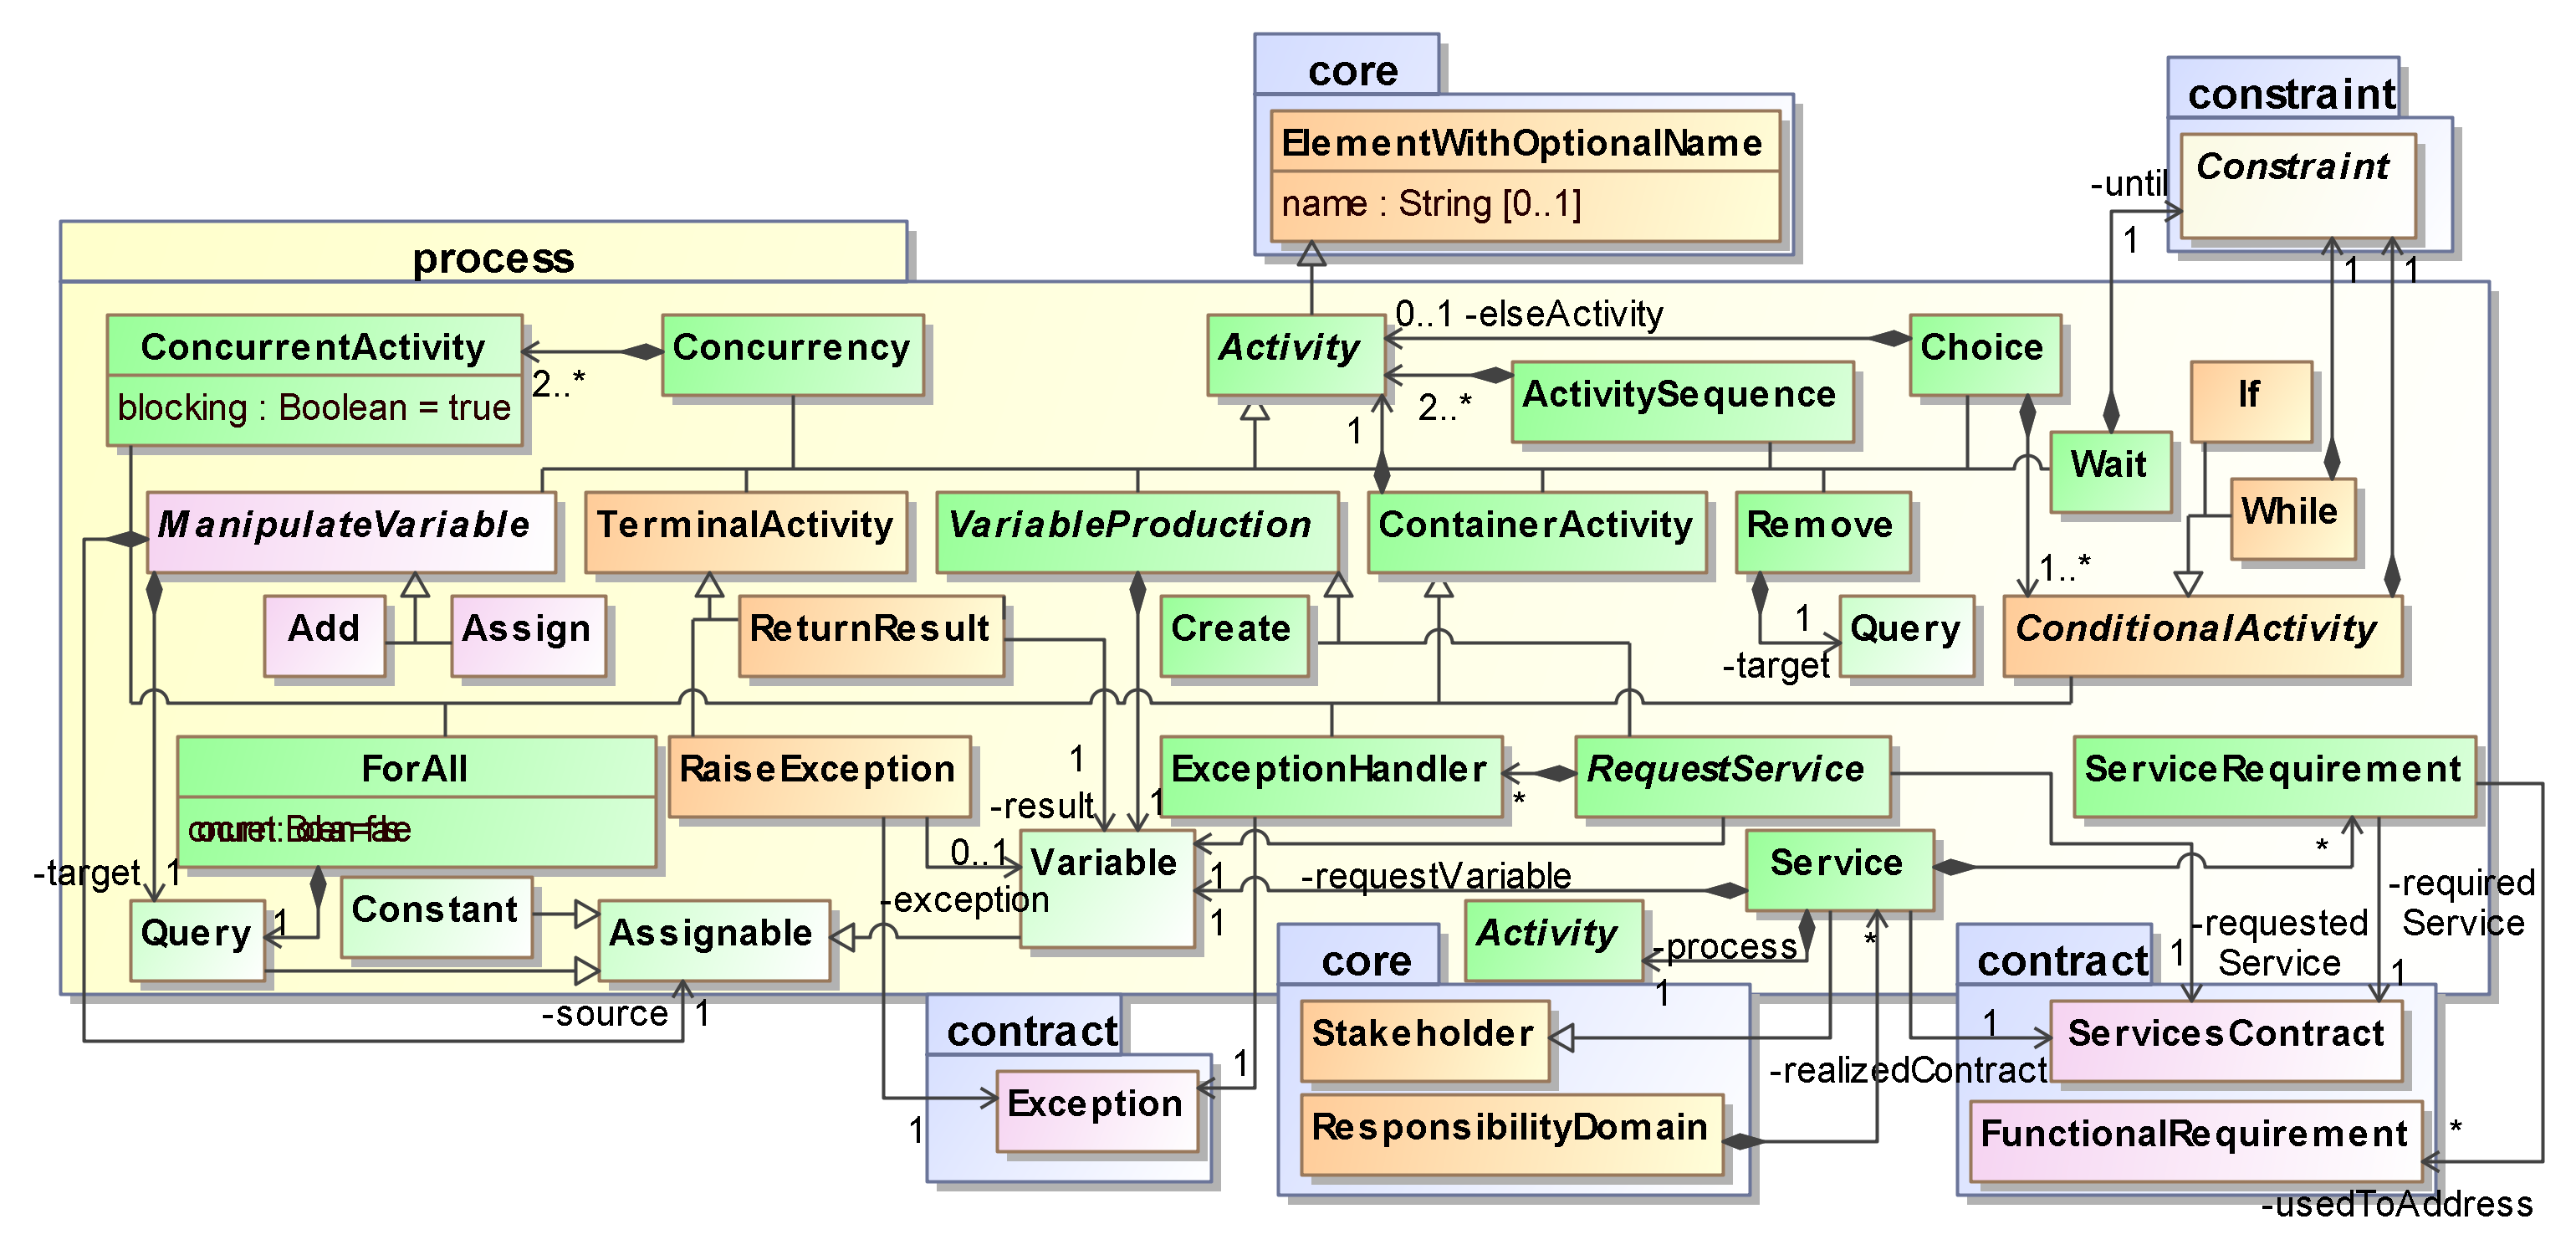
\includegraphics{process}
  \caption{The modeling constructs available for specifying services and processes in URDAD}
  \label{fig:processModule}
\end{figure}

The following listing illustrates how the specification of a service within the URDAD DSL text grammar.
\lstset{language=urdad,caption=Specifying a service in the textual URDAD DSL syntax.,label=serviceTextSyntax}
\begin{lstlisting}[numbers=left,escapechar=|]
Service enrollForPresentationImpl realizes enrollForPresentation receiving Variable enrollForPresentationRequest ofType EnrollForPresentationRequest
{
  use checkStudentSatisfiesEnrollmentPrerequisites toAddress (enrollmentPrerequisitesMet)
  use issueInvoice toAddress (financialPrerequisitesSatisfied invoiceIssued) 
  use performEnrollment toAddress (invoiceIssued)
   
  Process doSequential
  {
    create Variable checkStudentSatisfiesEnrollmentPrerequisitesRequest ofType CheckStudentSatisfiesEnrollmentPrerequisitesRequest               
    set Query OCL:"enrollForPresentationRequest.studentIdentifier" equalTo Query OCL:"checkEnrollmentPrerequisitesRequest.studentIdentifier"
    set Query OCL:"enrollForPresentationRequest.presentationIdentifier" equalTo Query OCL:"checkEnrollmentPrerequisitesRequest.presentationIdentifier"
                     
    requestService checkStudentSatisfiesEnrollmentPrerequisites with checkStudentSatisfiesEnrollmentPrerequisitesRequest yielding Variable checkStudentSatisfiesEnrollmentPrerequisitesResult ofType CheckStudentSatisfiesEnrollmentPrerequisitesResult
    choice
    {
      if Constraint enrollmentMeetsPrerequisitesMet OCL:"checkStudentSatisfiesEnrollmentPrerequisitesResult.enrollmentPrerequisitesMet = true"
        doSequential
        {
          ...
          requestService issueInvoice with issueInvoiceRequest yielding Variable issueInvoiceResult ofType IssueInvoiceResult
          {
            on FinancialPrerequisitesNotSatisfiedException raiseException FinancialPrerequisitesNotSatisfiedException
          }
	      ...
          requestService performEnrollment with enrollRequest yielding Variable performEnrollmentResult ofType PerformEnrollmentResult
          
          create Variable enrollForPresentationResult ofType EnrollForPresentationResult
          set Query OCL:"issueInvoiceResult.invoice" equalTo Query OCL:"enrollForPresentationResult.invoice"
          ...                       
          returnResult  enrollForPresentationResult
        }
      else raiseException EnrollmentPrerequisitesNotSatisfiedException
    }
  }
}                 
\end{lstlisting}

%---------------------------------------------------------------

\subsection{Process consistency}
\label{sec:processConsistence}

In order to assess the internal consistency of the metamodel, we mapped it onto a OWL-DL ontology using the TwoUse framework\cite{parreiras_using_2010}. The results are discussed in a paper discussing the URDAD-DSL which is currently under review. They show that within the limited reasoning capabilities of the generated description logic, the metamodel was found to be consistent.

Since URDAD is a general service-oriented analysis and design methodology, it can be applied to analyze the requirements and design of a service providing a technology-neutral analysis and design model for a service. We have done this and the process demonstrated that the URDAD metamodel and process are regenerated by the URDAD process itself. This demonstrates the internal consistency of the URDAD process itself.
